\chapter{Sistema Proposto}
\label{cap:Estrutura}

Para conceber a arquitectura do sistema de Monitorização de Rede orientado ao Processo (MRoP), foi necessário conhecer como os processos comunicam com o núcleo de forma a efectuar comunicações com o exterior.
Após conhecer a arquitectura de rede do \textit{Linux}, foi necessário compreender de que forma se processa a comunicação, bem como a monitorização de rede.

Neste capitulo irá ser apresentado a constituição do sistema de rede do \textit{Linux}, desde o momento em que a aplicação envia os dados, até ao momento em que estes chegam à interface de rede e vice-versa.
Como esta visão é muito abrangente, apenas serão focados os pontos essenciais da arquitectura.
Após esta visão geral do sistema de rede do \textit{Linux}, será apresentada a arquitectura do sistema (MRoP).


\section{Arquitectura de rede em \textit{Linux}}
\label{sub:network}

Um processo é uma instância de um programa, este num sistema multiprogramado partilha recursos do sistema com outros processos.
Os processos necessitam de comunicar com outros processos, para obter dados, de forma a completar as suas execuções.
Estas comunicações podem ser efectuadas dentro do mesmo sistema ou externas.
Em geral as comunicaçoes externas são efectuadas via rede, sendo necessário para isso criar canais de comunicação.
A(s) interface(s) de rede são partilhadas pelos diversos processos, sendo esta partilha efectuada pelo núcleo, pois apenas este é capaz de efectuar uma partilha correcta deste recurso.

A criação de canais de comunicação é efectuada através da chamada ao sistema \textit{socket}.

----------- --------- ----------- qualquer coisa sobre a Norma posix ------------

A chamada ao sistema \textit{socket} é efectuada para a criação do canal e dependendo dos parâmetros instânciados para este, varia o tipo e o protocolo utilizado.
Existe um agrupamento em familia de endereços (\textit{Address Family}), este podem ser para comunicação remota ou local.
As comunicações locais podem ser entre processos (\textit{AF\_UNIX}), ou entre processos e o núcleo (\textit{AF\_NETLINK}).
As remotas podem ser efectuadas sobre a internet, existindo também para estas uma familia própria, a \textit{AF\_INET}.
Os canais têm um conjunto de funções (\textit{API}) bem definidas para utilização e controlo, permintindo assim criar uma forma estruturada de comunicação.

Os administradores de sistemas necessitam de filtrar o fluxo de informação que circula nas suas redes, por isso têm sido desenvolvidos sistemas de filtragem de comunicações, também conhecidas com \textit{firewalls}.
Sendo o \textit{Linux} um sistema de operação utilizado em larga escala em ambientes de servidores, necessitou também deste controlo. Tem sido desenvolvido o \textit{NetFilter}, uma \textit{Firewall} que filtra o fluxo de dados que circula entre o sistema e a periferia deste, via rede.

Para além da filtragem do fluxo de dados, existe também um sistema de controlo do tráfego (\textit{Traffic Control}).
Este sistema permite ao administrador indicar quais os fluxos de dados prioritários, ou que necessitam de uma determinada largura de banda e assim efectuar uma reserva anticipada para estes.
Quer o \textit{NetFilter} como o \textit{Traffic Control} são ambos definidos dentro do núcleo.
 
Nas subsecções seguintes irão ser apresentados diferentes constituintes da estrutura de rede do \textit{Linux}, começando pelo processo em nível utilizador até aos controladores de interfaces de rede. As últimas duas subsecções apresentarão a visão geral do fluxo de um canal de comunicação, envio e recepção, respectivamente.

%Os processos em um sistema são instâncias de um programa, que partilha recursos físicos e lógicos da máquina.
%Os processos para aceder a alguns recursos, podem necessitar de efectuar comunicações com instâncias de outros programas, estes podem estar localizados na mesma máquina (processos locais), ou estar em outra máquina (processos remotos).

%Um processo para comunicar com outro através, utilizará as funcionalidades de rede do seu sistema de operação.
%Pois apenas este sabe gerir correctamente os recursos de rede.

 %Para isto um processo tem de efectuar o inicio da comunicação enviando alguns pacotes de inicio de sessão (caso o protocolo de comunicação necessite).
% Um processo em \textit{Linux} é uma instância de um programa que partilha recursos da máquina, físicos ou lógicos.
%\todo{muito pormenor}
% Os processos dentro do núcleo são instâncias de uma estrutura \textit{task\_struct} que contém diversos elementos pertencentes ao processo, tais como identificadores de processo, tabela de ficheiros abertos, zonas de memória atribuidas, permissões, etc.
 
% Um processo para utilizar as funcionalidades de rede necessita criar uma instância de um \textit{socket}, que fica referênciado através de um descritor de ficheiros (descritor de \textit{socket}).
% Tal como os ficheiros são acedidos em nível utilizador através de descritores os \textit{sockets} também são acedidos e manipulados através destes, apenas com chamadas ao sistema próprias para controlo e comunicação nestes canais.
 %Os \textit{sockets} são mapeados no sistema de ficheiros virtual, permitindo desta forma neste caso sobre a forma de \textit{sockets}, forma de comunicação sobre a rede.
% Estes descritores permitem ao processo identificar o \textit{socket}, para efectuar as comunicações.
 %Estas comunicações, bem como o estabelecimento destes canais de comunicação, são efectuadas através de chamadas ao sistema de operação.

%Falar aqui sobre qq coisa da estrutura de rede ... 
%Talvez tb imagem com um pouco da arquitectura ... básica 

%Falta falar sobre o netfilter ... sobre tc trafic control

%  Descrever um pouco esta parte ...
% Os canais de comunicação de rede estão organizados em familias de endereços, sendo a familia de endereços \textit{AF\_INET} utilizada para efectuar comunicações sobre a internet.
%Outras familias de \textit{sockets} existentes são \textit{AF\_NETLINK}, \textit{AF\_UNIX}, etc.
%A chamada ao sistema \textit{socket} é composta pela familia de endereços, pelo tipo e pelo protocolo.
%Desta forma generica é possível mapear diferentes tipos de comunicação, tais como \textit{INET} , \textit{NETLINK}, \textit{UNIX LOCAL}, em uma estrutura, o \textit{BSD socket}.

% A generalidade das aplicações utilizam os \textit{sockets} da familia \textit{AF\_INET}, para efectuar as suas comunicações sobre redes, sendo os principais tipos utilizados o \textit{INET\_STREAM} e \textit{INET\_DGRAM}.
% Estes dois tipos oferecencem canais orientados à conexão com estado e sem estado, respectivamente.


%Quando a chamada ao sistema \textit{socket} é efectuada, é criado uma nova instância de um socket e inicializados os respectivos campos com a informação dependente para a familia e tipo. 

%As principais chamadas ao sistema para estabelecer, terminar e comunicar sobre \textit{sockets} são: \textit{socket}, \textit{close}, \textit{connect}, \textit{bind}, \textit{listen}, \textit{accept}, \textit{send}, \textit{recv}, \textit{sendto} e \textit{recvfrom}. 


%Os file descriptors (socket descriptors) são os identificadores para os sockets. Os sockets são mapeados em ficheiros e estes em descritores de ficheiros. 

\subsection{Estrutura de um processo}
% ou recursos de rede de um processo

Um processo é a instânciação de um programa, sendo também uma unidade de escalonamento de execução (\textit{task}) no sistema.
Este consome recursos (físicos e lógicos), partilhados com outros processos num sistema multiprogramado.
O núcleo para cada processo gere uma estrutura, \textit{struct\_task}, onde estão identificados todos os recursos atribuidos a este.
Esta estrutura contém apontadores para diversos recursos tais como: zonas de memória requisitadas, canais abertos (ficheiros, \textit{sockets}, entre outros), contabilização de utilização de \textit{cpu}, apontadores para a sua àrvore geneológica (pai, irmãos e filhos), etc.

Os apontadores para a sua árvore geneológica são: apontador para o pai (o processo que efectuou um \textit{fork}, para lhe dar origem), a lista de irmãos e de descententes.
Cada um dos elementos da lista, ou o pai, são também eles estruturas do tipo \textit{task\_struct}, o que permite navegar pela árvore geneológica do processo.

Um dos recursos partilhados pelos diferentes processos é o acesso à rede, permitindo desta forma a comunicação com o exterior.
Para serem efectuadas comunicações é necessário a alocação de canais de comunicação, por isso o sistema de operação tem uma \textit{API} de comunicação que permite a criação, destruição e a utilização destes.
Quando um processo cria um canal, o sistema devolve-lhe um identificador.
Este identificador serve para o processo referênciar o canal, dentro do núcleo, de forma a efectuar as suas futuras comunicações, bem como o controlo deste.
Dentro do núcleo, este identificador é gerido na estrutura que identifica os canais abertos, pelo processo.

A estrutura de canais abertos, permite abstrair qual o canal que foi aberto, se foi um ficheiro, um socket, um \textit{pipe}, etc.
Para reconhecer qual o tipo do canal aberto existem algumas funções especificas que analisam qual o tipo e permite efectuar diferentes tipos de operações consoante o canal.
Por exemplo ao manipular um ficheiro existe a possibilidade de avançar e recuar, sobre um determinado ponto dentro do ficheiro.
Esta situação não faz sentido quando se controla um \textit{socket} ou um \textit{pipe}, pois as comunicações nestes são destruidas quando consumidas, enquanto que isso não acontece num ficheiro.
 

%Um processo para executar tem de ser carregado para memória e posteriormente ser agendado para execução através do escalonador de processos do núcleo.
% Um processo para o núcleo é uma estrutura com a informação sobre as zonas de memória, descritores de ficheiros abertos, informações sobre os tempos de execução, informações sobre a hierarquia de processos pertencentes a este, etc.
% Nos descritores de ficheiros abertos são também incluidos os descritores de \textit{sockets} abertos para comunicação. 

% Dentro do núcleo do linux a estrutura que tém a informação sobre um processo (\textit{task}), é a \textit{struct task\_struct}. 
% Nesta estrutura existe a informação sobre quais os ficheiros que a aplicação abriu.
% Como os \textit{sockets} são mapeados sob a forma de ficheiros, estes também se encontram nesta estrutura.


\subsection{Sockets e suas familias}
\label{sub:sockets}

Como anteriormente referido em \ref{sub:network}, um processo para comunicar via rede, tem de criar um canal.
Os canais são criados para comunicar com diferentes pontos, uns localmente e outros com o exterior.
Desta forma os canais são diferentes e apesar das acções que podem ser efectuadas serem comuns, o meio de transmissão é diferente e por isso diferentes formas devem ser utilizadas.

Os \textit{sockets} podem ser agrupados pelas familias de endereços \textit{Address Family}, que permitem especificar qual a forma de comunicação utilizada (local ou remota).
Para caracterizar o canal não é apenas necessário a especificação da familia, é também necessário especificar o tipo de canal e o protocolo que se irá utilizar.
Diferentes combinações de valores para estes parâmetros, permitem especificar canais com diferentes funcionalidades.

Nas subsecções seguintes irão ser apresentadas diferentes familias de endereços suportadas no núcleo do \textit{Linux}, tendo especial ênfase nas familias \textit{INET}, \textit{NETLINK} e \textit{PACKET}.


%Como já foi indicado em \ref{sub:network}, um processo para comunicar tem de utlizar um \textit{socket}.
% Os \textit{sockets} para se diferenciarem devido às suas diferentes utilidades são definidos em  familias de endereços.
% Os \textit{sockets} para comunicação de internet utilizam o domínio \textit{AF\_INET}, que permite utilizar diferentes tipos de protocolos, tais como \textit{UDP} e \textit{TCP}.
% Estes protocolos são utilizados pela generalidade das aplicações quando necessita de comunicar com outro processo que utilize os mesmos protocolos de comunicação.


%Address Family para o INET, internet sockets para ipv4 e AF\_INET6 para ipv6

\subsubsection{AF\_UNIX}

Esta familia de \textit{sockets} é utilizada para efectuar a comunicação entre processos dentro da mesma máquina.
É um dos sistemas de \textit{Inter Process Communication (IPC)}, utilizado em sistemas Unix.
Permite utilizar um ficheiro no sistema de ficheiros, como um canal de comunicações.

\subsubsection{AF\_NETLINK}


\subsubsection{AF\_INET}
\label{subsub:af_inet}

\textit{AF\_INET} é a familia de endereços utilizada na comunicação através da \textit{internet}, utilizando para isso o protocolo \textit{IP versão 4} (ver figura \ref{}

 (ainda tem de ser colocada stack tcp ip).

A estruturação por camadas permite que a implementação de protocolos seja efectuada de forma mais rápida e simples.
Existem diferentes vários protocolos de nível transporte sobre \textit{IPv4}, sendo os mais utilizados o \textit{TCP} e \textit{UDP}.
A criação de canais sobre o nível de transporte é efectuado utilizando a chamada ao sistema \textit{socket}, indicando como valores \textit{SOCK\_STREAM} ou \textit{SOCK\_DGRAM}, respectivamente, para o parâmetro tipo.
Cada protocolo tem a sua especificidade, permitindo assim efectuar comunicações de forma distinta.
O \textit{TCP} é utilizado para canais que necessitem de efectuar comunicações sem perdas de pacotes.
Para este protocolo é efectuado um controlo na transferência e recepção dos pacotes, permitindo adequar o ritmo de transmissão ao meio subjacente.
O \textit{UDP} é um protocolo mais leve que o \textit{TCP}, pois não utiliza o controlo anteriormente mencionado, sendo habitualmente utilizado quando existe a possibilidade de perda de pacotes durante a transmissão, ou quando o controlo da retransmissão de pacotes é efectuada em camadas superiores.

Para além destes protocolos existe também o \textit{SOCK\_RAW}, que permite acesso directo ao nível rede.
Este protocolo permite a criação de um canal que comunica directamente com o nível rede, da pilha de protocolos \textit{TCP/IP}, permitindo assim executar protocolos de comunicação em nível utilizador.

\subsubsection{AF\_PACKET}
\label{subsub:af_packet}

A familia \textit{AF\_PACKET} permite comunicar directamente com o controlador de rede, permitindo assim efectuar a monitorização de rede.
Tal como em anteriores familias apresentadas, esta familia permite definir diferentes formas de comunicação, em função do tipo e protocolo associados ao \textit{socket}.
A utilização destes \textit{sockets} requer uma autorização de \textit{CAP\_NET\_RAW}.
Esta verificação previne que utilizadores não autorizados possam monitorizar, ou injectar pacotes na rede, influenciando o comportamento desta.
Como permite enviar pacotes directamente para o controlador de rede, uma das utilizações é a implementação de protocolos de rede em nível utilizador, .
A utilização de canais da familia \textit{AF\_PACKET} é frequentemente utilizado para sistemas de detecção de intrusos, dado que permite analisar os pacotes e detectar falhas na correcta formatação destes.

Como a obtenção dos pacotes por estes canais, é efectuada primeiro que a recepção dos dados pelas aplicações, é possível obter mais pacotes que aqueles que a aplicação recebe.
Por isso se o \textit{NetFilter} bloquear a recepção de alguns pacotes, as aplicações não os irão receber, mas, este canal já os terá recebido para análise.
%Esta situação é devida ao posicionamento do \textit{NetFilter} em relação à monitorização de rede.
%No entanto ficaram visíveis à monitorização pois esta é efectuada antes de chegar aos \textit{Hooks} do \textit{netfilter}.
 
%Podem ser utilizados dois tipos \textit{SOCK\_DGRAM} ou \textit{SOCK\_RAW}.
 
%A utilização destes \textit{sockets} permitem a implementação de protocolos de rede, sem recorrer à \textit{stack} de protocolos IP dentro do núcleo.
% Para além desta funcionalidade esta é a forma de capturar os pacotes que circulam na interface de rede, permitindo assim efectuar uma análise do tráfego.

Como todos os pacotes recebidos pela interface(s) de rede são recebidos por este canal, existe a necessidade de efectuar uma cópia destes e fornece-los à aplicação em nível utilizador.
Esta monitorização implica um peso extra na computação, por isso diversas técnicas tem sido desenvolvidas para minimiza-lo.
A utilização de \textit{lazy cloning}, isto é, apenas efectuar a cópia caso seja realmente necessária, permitindo assim diminuir a perda de eficiência do sistema quando está a monitorizar os pacotes de rede.
A cópia do pacote é efectuada caso a avaliação do filtro indique que este deve ser copiado, caso contrário é terminada a execução em relação a esse pacote.

% Por isso primeiro são avaliados para o processo de captura, caso sejam para captura a função \textit{blah blah} efectua a cópia da estrutura sk\_buffer e serão então adicionados ao \textit{ring buffer}.
% Se no \textit{ring buffer} não existir espaço para o número de bytes que devem ser capturados, é então descartado a cópia (libertado o espaço) e incrementado o valor de pacotes descartados pelo núcleo de sistema.


\subsection{NetFilter}

O sistema de operação \textit{Linux} tem um sistema de \textit{firewall} que permite controlar os acessos dos processos aos sistemas de comunicação de rede.
 Este sistema é o \textit{NetFilter}, está presente no núcleo do sistema operação permitindo controlar o fluxo de dados dos processos para as interfaces de rede, bem como no sentido oposto.
 O \textit{NetFilter} está presente na \textit{stack TCP/IP} em 5 pontos apenas e desta forma consegue de uma forma simples controlar o fluxo dos dados.
 O \textit{NetFilter} pode ser controlado pelo \textit{iptables}, uma ferramenta em nível utilizador que através de regras define o acesso dos dados das comunicações rede.

\subsection{Traffic Control}

------------------------------------------------------------------------------------------------------------
 Dentro do núcleo do \textit{Linux} para além da \textit{firewall NetFilter} existe um mecanismo de controlo sobre os dados que circulam nas interfaces de rede.
 O principal propósito deste sistema é controlar a transmissão de dados, \textit{egress data transfer}.
 Quando os protocolos de nível 3 vão enviar os dados, para a camada de nível 2, estes são armazenados em \textit{QDisks} para posteriormente serem enviados.
 Com a necessidade de diferenciar os diferentes tipos de dados os administradores de sistemas podem diferenciar o trafego e armazená-lo em diferentes \textit{QDisks}, de forma a poder efectuar \textit{Quality of Service}.
Apesar de ter estrutra para controlo dos dados que chegam da interface de rede o principal propósito é controlo do dados que saem através das interface de rede.
------------------------------------------------------------------------------------------------------------

No núcleo para além do \textit{NetFilter}, que controla o fluxo de dados na rede, existe o \textit{Traffic Control} que efectua o escalonamento da transferências de dados para o exterior da rede.
O escalonamento do tráfego de rede é particularmente importante para os Administradores de rede, pois permite gerir de forma eficiente a largura de banda da interface de rede.
Como a largura de banda é um recurso limitado, a sua gestão é particularmente importante para os Administradores de rede.
Através do \textit{Traffic Control} é possível gerir o fluxo de dados de saída da interface de rede.
A gestão é efectuada através de regras definidas pelo Administrador, que permitem efectuar a diferenciação do tráfego de rede através da definição de classes.
É possível afectar diferentes algoritmos de escalonamento de forma a efectuar uma gestão da rede mais eficiente.
As regras são definidas em função da largura de banda, ou do ritmo de envio.

Quando um pacote \textit{IP} está prestes a ser enviado pela função \textit{ip\_output}, é enviado para o \textit{Traffic Control}, onde o pacote é marcado com a respectiva \textit{tag} da respectiva classe, para posteriormente ser adicionado ao \textit{QDisk} correspondente à sua classe.
O \textit{QDisk} é a estrutura de suporte à transmissão de dados efectuada pelo \textit{Traffic Control}, onde cada elemento desta estrutura é um \textit{sk\_buff}.


\subsection{Interfaces de rede}

A interface de rede é o dispositivo que envia e recebe os pacotes de dados na rede.
Do ponto de vista da interface de rede, apenas executa pedidos de interrupção ao processador.
O controlador de rede faz a ponte entre as funcionalidades de rede do núcleo e a interface de rede.

O núcleo mantém a informação sobre as interfaces de rede, inicializadas pelos seus controladores, e que mesmo não estando activas, constantam de uma lista duplamente ligada de \textit{net\_devices}.
Em cada posição desta lista existe a informação referente a uma interface de rede e suas configurações, nomeadamente a informação sobre o seu endereço ip ou o seu \textit{mac address}, no caso de interfaces \textit{ethernet} ou mapeadas sobre \textit{ethernet} (como o caso de interfaces ponto-a-ponto).

No registo de um novo controlador de interface de rede definem-se as operações a executar em determinados eventos, tais como, recepção e/ou transmissão de frames, remoção da interface, etc.
Estas operações são definidas através de uma interface comum, a \textit{struct netdev\_ops}, permitindo definir a \textit{API} das interfaces de rede.

Falar sobre os controladores das interfaces de rede, que definem um conjunto de funções para serem desencadeadas em determinados pontos do envio ou recepcao de frames ... ndo (netdevice operations) 
 
\subsubsection{Estrutura de um sk\_buff}
\label{subsub:sk_buff}

Os dados envolvidos no fluxo de comunicação e utilizados pelos controladores são os \textit{socket buffers}, estruturas do tipo \textit{sk\_buff}.
Esta estrutura contém diversos elementos, sendo alguns dos principais elementos os apontadores para a estrutura de rede do controlador, apontadores para secoções do pacote (os diversos cabeçalhos pertencentes ao nível de rede e transporte), bem como distância ou tamanho dos espaços alocados para estes e outros apontadores.
Uma estrutura com os diferentes cabeçalhos necessários à sua transmissão ou recepção.
Existem 4 apontadores para endereços de memória dentro da estrutura que definem os endereços de inicio e fim do pacote, bem como dos cabeçalhos.
Falta boneco com esta informação ... fica mais realista.

\subsection{Recepção de dados}
---------------------------------------OLD-----------------------------------------------------------
A chegada de um pacote de dados à interface de rede desencadeia uma acção de interrupção da actividade do processador, permitindo quer este seja transferido para o sistema o mais cedo possível.
Esta interrupção é efectuada através de um \textit{irq} pré-definido entre o controlador e a interface de rede. As interrupções são atendidas no processador desligando a atenção a todas as outras interrupções provenientes de outros dispositivos. %esta frase está ruim ...
O processador deve estar o menor intervalo de tempo possível com as interrupções desligadas, antes de retornar da interrupção o sistema agenda a execução de uma função que irá terminar a recepção do pacote para a camada correcta da \textit{stack TCP/IP}.%ainda falta falar sobre DMA, interrupt mode too exclusive deve ser breve, encaminhar pelo processamento da stack tcp/ip 

No processo de recepção da \textit{frame} é verificado se existem \textit{sniffers} registados, caso existam é passada uma referência sobre a frame, de forma a efectuar apenas a cópia da frame quando necessária.
Esta situação é devida à possível existência de um filtro sobre a \textit{frame}, em que se não for necessário capturá-la, a cópia dos dados seja desnecessária, permitindo efectuar trabalho útil.

Faltar falar que a frame segue para a stack tcp ip de forma normal ...

Falta falar sobre o netfilter ... firewall do linux que existem 5 pontos de "entrada" onde existe algumas verificações .... 

Faltar indicar que o processo está bloqueado à espera de input que lhe é copiado entre o nucleo e o processo em nivel utilizador por meio de o kiovec (talvez kernel io vector ...) 


A variável global \textit{ptype\_base} do núcleo é uma tabela de dispersão aberta, que contém os tipos de controladores de protocolos de rede. Os diferentes protocolos endereçam uma função que recebe o pacote e sabe o que fazer com ele, passando pela \textit{firewall netfilter} terminando na cópia dos dados dos \textit{buffers} do núcleo para os do processo, que ficou bloqueado numa lista de espera através da chamada ao sistema de operação \textit{recv}, \textit{recvfrom} ou \textit{recvmsg}.
----------------------------------------END OF OLD----------------------------------------------------

O processo de recepção de pacotes pelas aplicações através de interfaces de rede, atravessa as diversas componentes apresentadas anteriormente em .... , ... e ... .

O sistema de monitorização de rede opera de forma opoca à normal utilização de rede, pelas aplicações.
Quando um pacote chega à interface de rede, esta envia um pedido de interrupção da computação ao cpu, de forma que este atenda o pedido da interface de rede.
Neste ponto é desligada a atenção do processador a novas interrupções e a computação passa para o controlador da interface de rede.
Uma vez que a atenção do processador a novas interrupções está desligada, a computação deve ser o mais breve possível de forma a poder ligar novamente a atenção do processador a interrupções, para que o normal funcionamento seja retomado, por isso apenas a computação crítica é efectuada e é registada a necessidade de invocação de um \textit{softirq}, para que seja terminado o tratamento dos pacotes que chegaram à interface.
A invocação do \textit{softirq} é utilizado de forma que a computação seja terminada e que possam ser atendidos novos eventos no processador, o que permite uma maior actividade por parte deste.
O \textit{softirq} escalonado opera sobre o pacote recebido pela interface de rede, de modo que seja possível analisá-lo.
Antes de ser analisado pelo \textit{packet handler} respectivo, este é passado para os \textit{sniffers} registados no sistema.
Estes \textit{sniffers} são a forma de monitorizar a rede

\subsection{Transmissão de dados}

Uma aplicação em nível utilizador transfere dados sobre a rede através de chamadas ao sistema de operação, sendo que estas podem ser \textit{send}, \textit{sendto}, \textit{sendmsg}.
 Neste ponto de entrada os dados tem de ser copiados e efectuadas diversas verificações sobre estes, após estas verificações são utilizadas estruturas e funções através da \textit{stack TCP/IP} e fluir pela \textit{firewall netfilter}.
 Os dados gerados pelas diversas camadas da \textit{stack} são agregados numa estrutura \textit{sk\_buffer} para ser adicionados a uma fila para ser enviados pela ferramenta \textit{traffic control}.
 Quando esta ferramenta irá enviar os dados para o controlador é passada a referência sobre este pacote para os \textit{sniffers} registados, sendo apenas efectuada uma cópia dos dados caso o pacote seja recolhido para maior análise. Os dados passados ao controlador da interface de rede são então transferidos para a interface de rede, e daí para o seu destino.

Quando a aplicação está a executar e efectua uma chamada ao sistema de operação, o sistema muda de modo e executa dentro do núcleo "em nome da aplicação".
 Durante parte da execução da chamada ao sistema de operação é possível referenciar qual o processo que efectuou a chamada, pois caso a chamada seja sincrona, é agendada um processamento sobre os dados e a aplicação fica bloqueada à espera de ser re-escalonada através da função \textit{schedule}.
 O sistema de ficheiros mantém a referência sobre quais os ficheiros/sockets abertos para cada processo e é possível obter qual o processo a que cada descritor de ficheiros pertence. % back pointers ... nos sockets ... binded de uma porta a um processo ... pode nao ser a chamada bind ... 

\section{Desenho e arquitectura do MRoP}
\label{sec:mrop_architecture}

O sistema proposto foi desenvolvido procurando cumprir os seguintes requisitos:
\begin{itemize}
\item permitir seleccionar as comunicações envolvendo apenas um processo (ou um conjunto de processos);
\item manter a compatibilidade com o sistema já existente, estendendo a sua funcionalidade;
\item procurar minimizar eventuais percas de desempenho;
\item a implementação deve envolver poucas alterações ao código do sistema, para facilitar a sua manutenção e evolução com as novas versões do sistema Linux.
\end{itemize}

Para tal, o sistema criado está dividido em 4 componentes principais (ver figura \ref{arquitectura}).
A função de filtragem, invocada por um \textit{hook} que estende o \textit{LSF}, permite que apenas o tráfego do processo alvo seja analisado pelo restante sistema de fitragem do LSF.
Uma componente de instrumentação das chamadas ao sistema (ou outras funções contidas no sistema de rede) que actualiza o repositório de dados onde é mantido o estado das interacções via rede do(s) processo(s) alvo.
Existe ainda um sistema para controlo/configuração e para obter informação do estado da monitorização.

\begin{figure}[htbp]
\begin{center}
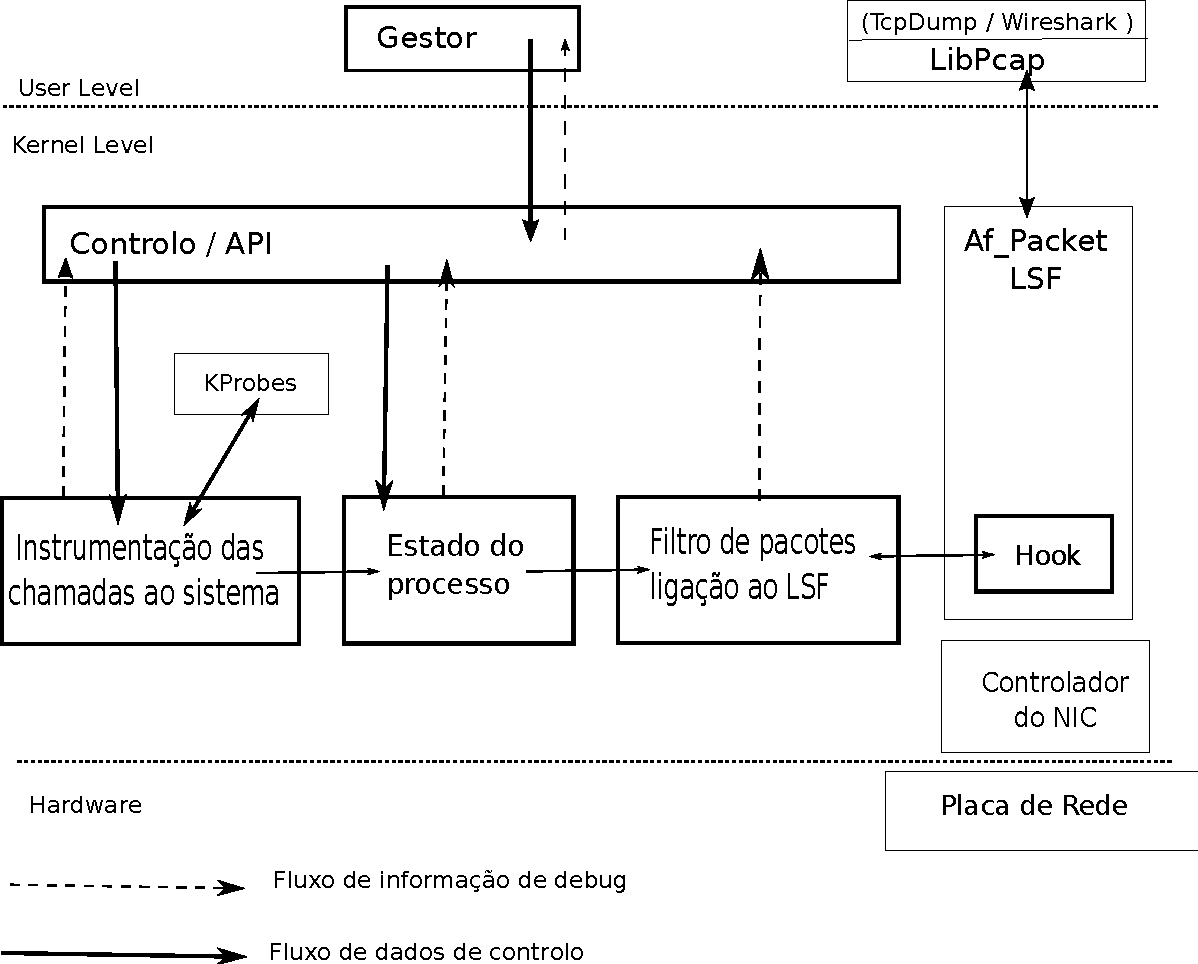
\includegraphics[scale=0.5]{interface.pdf} 
\caption{Arquitectura da solução}
\label{arquitectura}
\end{center}
\end{figure}


Este sistema permite que sejam capturados os pacotes de rede de um processo, sem que exista um conhecimento prévio sobre o(s) protocolo(s) ou portas utilizadas.
 A utilização de um sistema de instrumentação do núcleo foi necessária apenas para monitorizar as chamadas envolvendo \emph{sockets} e identificar o processo responsável, permitindo desta forma obter e manter permanentemente actualizada a informação sobre o estado respeitante ao processo alvo.
 De forma a minimizar a redução de desempenho, todo o sistema foi desenvolvido dentro do núcleo do \textit{Linux}, sem alterações nas interfaces já existentes.
 Assim, ferramentas de façam uso da biblioteca \textit{LibPcap}, como o programa \textit{tcpdump} ou suas variantes, podem beneficiar desta extensão sem qualquer alteração e sem impacto relevante no seu desempenho.

---------------------------------------------------------------------------------------------------------

A arquitectura foi pensada para ser executada de forma ortogonal ao sistema utilizado.
 Desta forma não existe a necessidade de recompilar programas antigos.
 Para além desta situação novas aplicações podem utilizar esta ferramenta de forma transparente.

Esta ferramenta foi desenvolvida para os processadores x86 e x86\_64 pois nestas arquitecturas existe suporte para o sistema de monitorização KProbes \ref{}, sendo esta a unica dependência especifica que a ferramenta irá ter.

As diferentes partes da ferramenta foram desenvolvidas de forma a poderem ser modificadas em separado permitindo um melhor aproveitamento da modularização.
Este módulo foi desenvolvido em 4 subpartes. 

---------------------------------------------------------------------------------------------------------


\subsection*{Instrumentação das chamadas ao sistema de rede}
\label{sub:mon_syscalls}

Um ponto importante deste sistema, constituiu na garantia que todas as interacções desencadeadas por um processo com o exterior fossem detectadas. Para tal, foi necessário recorrer à monitorização das chamadas ao sistema de rede ao nível do Kernel, permitindo, assim, minimizar as cópias de dados e trocas de contexto. Tirando partido da utilização do sistema de monitorização KProbes foi possível realizar a monitorização sob o pequeno conjunto de chamadas ao sistema relevantes, nomeadamente: sendto, recvfrom, bind, accept, connect e close.
 Na realidade verificou-se a chamada ao sistema close, ao ser utilizada intensivamente por todo o sistema de ficheiros, poderia degradar desnecessariamente o desempenho. Desta forma, decidiu-se aplicar a monitorização à função interna \texttt{sock\_close}, garantindo apenas a monitorização das chamadas close sobre os sockets, reduzindo significativamente o número de eventos face às chamadas ao sistema do \texttt{close}.

\subsection*{Estado do processo}
\label{sub:data_repository}

O estado dos portos TCP e UDP em uso pelo processo alvo é mantido num repositório de dados, e permanentemente actualizado pelo módulo anterior. 
 A estrutura dados escolhida para o efeito, para produzir o repositório pretendido, baseia-se numa árvore \textit{Red and Black} já disponível no núcleo do sistema. O conteúdo de cada folha da árvore é uma estrutura com duas listas de elementos, cada uma contendo endereços IP utilizados pela aplicação. A chave de indexação das folhas é o número do porto, desta forma a árvore poderá conter 65535 elementos. No pior caso, a procura de um porto na árvore necessitará de efectuar 16 iterações.
%\td{conteúdo? ip, interface, porto udp, porto tcp, etc??}
  O uso deste tipo de estrutura permite obter um bom compromisso entre o tempo de acesso à estrutura e a quantidade de memória utilizada.


\subsection*{Filtro de pacotes}
\label{sub:packet_filter}

A função de filtragem  implementada neste sistema assenta no estado do processo alvo, mantido pelos módulos anteriormente descritos.
Através da extensão do LSF com um hook, quando ligado, este invoca esta filtragem que devolve ao LSF se o pacote deve ser logo ignorado (não envolve nenhum dos portos do processo alvo) ou se se deve continuar a avaliar as restantes regras de filtragem definidas.
 Mantém-se assim a compatibilidade e continua-se a tirar partido dos benefícios da utilização do Linux Socket Filter.

Para continuar a ser opaco para os diferentes sistemas de monitorização/captura de rede foi necessário colocar um ponto de ligação entre o sistema actual e o módulo desenvolvido.
 Quando não existe uma ligação(\textit{Hook}) activa, existe apenas um ligeiro decréscimo no desempenho, este deve-se apenas à verificação da existência se esta ligação está activa.
 Caso a ligação esteja activa o fluxo de controlo é passado para a função de filtro definida no módulo.
 Desta forma é possível criar funções que permitem controlar o fluxo de dados que devem ser processados ou descartados

Necessidade de registar um \textit{hook} para aceder directamente à função de filtro.
 Caso este \textit{hook} não esteja ligado o \textit{overhead} introduzido será o de um teste para verificar se existe ligação ou não.
 No caso de não existir a ligação a este \textit{hook} o sistema comporta-se de forma a utilizar apenas o sistema anterior.

O sistema interage também com o \textit{LSF} pois existe uma conjunção entre o filtro definido pelo utilizador e a captura do tráfego da aplicação a ser monitorizada.


\subsection*{Controlo e Informação}
\label{sub:data_information}

Para facilmente controlar e configurar o sistema desenvolvido foi definida uma interface baseada em ficheiros virtuais (DebugFS).
 Estes ficheiros estão apenas acessíveis ao utilizador \textit{root}, controlando o acesso por parte dos utilizadores da máquina ao sistema de monitorização.
 Os ficheiros de controlo definidos foram \textit{option}, \textit{pid}, \textit{ppid} e \textit{tgid}.
 O primeiro ficheiro permite controlar a análise e a informação da árvore.
 Dependendo do valor a escrever em \textit{option} o sistema poderá proceder a uma análise dos \textit{sockets} do processo (identificado em \textit{pid, ppid, tgid}), e carregar essa informação para a àrvore do estado do processo, bem como poderá remover todos os elementos da àrvore se for essa a opção escrita para o ficheiro.
 Como foi indicado os restantes ficheiros permitem definir o(s) processo(s) a monitorizar.
 Pode ser indicado um processo ou todos os processos de um grupo.
 Os ficheiros de informação \textit{filter\_stats}, \textit{syscalls\_calls\_stats} e \textit{tree\_info} foram definidos para obter estatísticas dos pacotes analisados e das entradas/retornos das funções instrumentadas, bem como dos elementos presentes na árvore (dados dos sockets activos do processo).

\subsubsection*{Mais info}
%a não utilização de ioctl para o debug ... 
A estratégia foi separar os diferentes componentes e a criação de um módulo de \textit{debug} para que pudesse existir uma forma de acesso à monitorização por parte do nível de utilizador, sem que exista a necessidade de criar ou alterar chamadas ao sistema ou suas opções.



\section{Conclusão}

Algumas ideias para concluir este capitulo ...

